As described earlier, the system ultimately goes to the absorbing extinct state.
The time in which this happens is a random variable, the mean of which is the mean time to extinction $\tau_e$.
For one-species systems it is well known how to exactly solve the mean time to extinction for a one step birth and death process \cite{Nisbet1982,Palamara2013}.
The mean time of extinction, for a population of size $n$, is
\begin{equation}
\tau(n) = \frac{1}{d(1)} \sum_{i=1}^n \frac{1}{R(i)} \sum_{j=i}^N T(j)
\label{analytic_mte}
\end{equation}
where
\begin{equation*}
R(n) = \prod_{i=1}^{n-1} \frac{b(i)}{d(i)} \quad \textrm{and} \quad T(n) = \frac{d(1)}{b(n)}R(n+1).
\end{equation*}
Combining equations \ref{birth} and \ref{death} with the solution for the mean time to extinction \ref{analytic_mte} we obtain a complicated analytical expression in the form of a hypergeometric sum.
A typical trajectory starting from $n$ goes first to the deterministic fixed point $K$ and fluctuates about that point before a large fluctuation leads to its extinction.
%The mean time to extinction depends on the initial population size $n$, however
Since the time for the population to reach carrying capacity is insignificant compared to the extinction time, the MTE is largely independent of the initial population, and we write $\tau (n) \approx \tau_e$ for all $n$.
It is well known that $\tau_e$ goes like $e^K$ \cite{Ovaskainen2010} and this is indeed what we observe, see supplemental information.
What is less well known is the dependence on the hidden parameters, which we detail below.
\iffalse
%%%%%%%%%%%%APPENDIX%%%%%%%%%%%%%%
\begin{figure}[ht!]
\centering
\includegraphics[width=0.6\textwidth]{MTE_vsK (4 lines at lowlow, highhigh, highlow, lowhigh}
\begin{figure}[ht!]
\centering
\includegraphics[width=0.6\textwidth]{MTE_QvsD_K100_100}
\caption{\emph{Lorum ipsum} So many words..} \label{otherlabel}
\end{figure}
\end{figure}
%%%%%%%%%%%%%%%%%%%%%%
\fi
\begin{figure}[ht!]
\centering
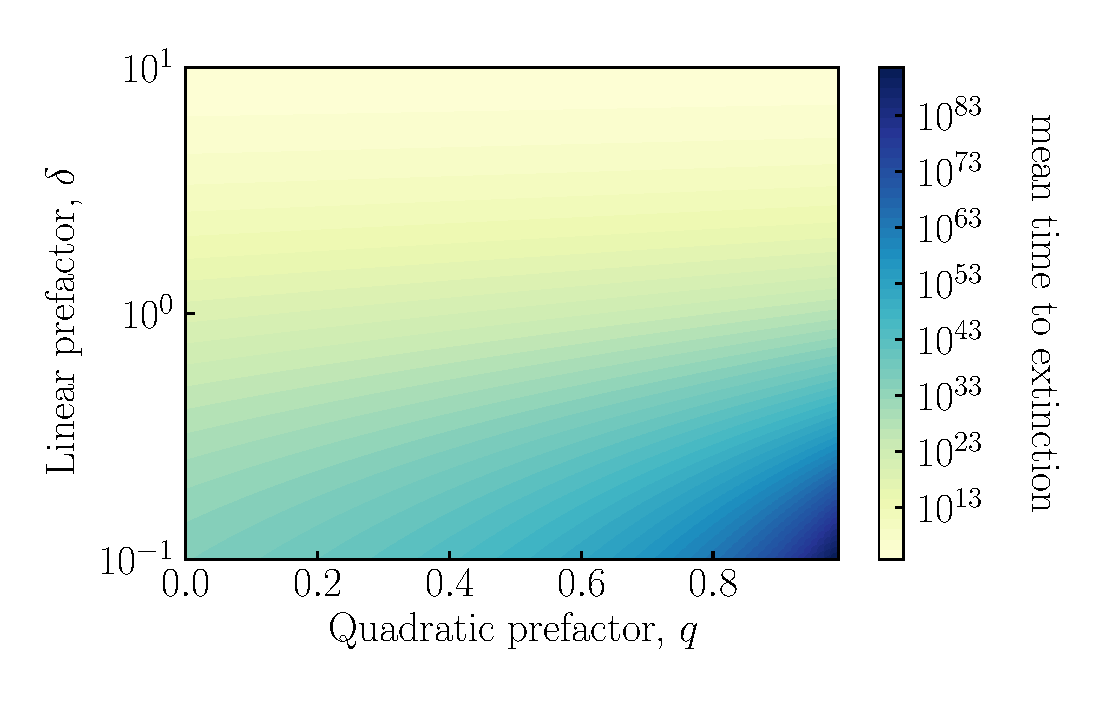
\includegraphics[width=0.6\textwidth]{Figure2}
\caption{\emph{Exploring the mean time to extinction in the parameter space} Recall that $q$ shifts the nonlinearity between the birth and death rates: for $q=0$ the nonlinearity is purely in the death rate, for $q=1$ nonlinearity appears only in birth. The birth and death rates are increased simultaneously with $\delta$.} \label{mteCP}
\end{figure}

The numerical results of this finite sum are summarized in Figure \ref{mteCP}.
It is evident that the MTE depends on the values of $\delta$ and $q$, parameters that appear in the births and deaths but do not appear in the deterministic equation.
%Increasing $\delta$ causes $\tau$ to decrease whereas increasing $q$ has the effect of increasing $\tau$.
%We can synonymously describe these phenomena in the language of population dynamics:
Increasing the scaling of the linear terms $\delta$ in birth and death rates has a tendency to decrease $\tau_e$.
On the other hand, shifting the nonlinearity from the death to the birth rate, in other words increasing $q$, causes an increase in $\tau_e$.
Note however that the effect of $q$ is magnified for smaller values of $\delta$ and weaker for larger values of $\delta$: see Figure \ref{mte}.

\begin{figure}[ht!]
  \centering
  \subfloat[\emph{Varying $\delta$}]{\includegraphics[width=0.5\textwidth]{Figure3-A}\label{mte:delta}}
  \hfill
  \subfloat[\emph{Varying $q$} ]{\includegraphics[width=0.5\textwidth]{Figure3-B}\label{mte:q}}
  \caption{\emph{Mean time to extinction for varying $\delta$ and $q$} Each line represents a slice in Figure \ref{mteCP}: Figure \ref{mte:delta} are vertical slices which show how, for different values of $q$, the $\delta$ affects $\tau$. Similarly Figure \ref{mte:q} are horizontal slices which show how, for different values of $\delta$, the $q$ affects $\tau$. As in Figure \ref{qsd}, lightness of the line indicates an increase of \ref{mte:delta} $q$ and \ref{mte:q} $\delta$}
  \label{mte}
\end{figure}
